
\section{Introduction}
\label{sec:api}

Our SIGGRAPH Asia paper {\em GPU-accelerated Path Rendering} \cite{KilgardBolz2012}
describes a system for accelerating vector graphics on GPUs. NVIDIA has
implemented the system and has been shipping the functionality for its GeForce and Quadro GPUs since the summer of 2011.
We refer the reader to that paper for the motivation and technical underpinning
of the {\tt NV\_path\_rendering} \cite{NVpr} OpenGL extension.  In particular, that
paper explains our ``Stencil, then Cover'' (StC) approach to filling and stenciling paths.

In this annex to the forementioned paper we explain the programming interface in
more detail.  The intended audience for this annex is developers
evaluating and learning to program {\tt NV\_path\_rendering}.  You should
be familiar with the OpenGL \cite{OpenGLspec} programming interface.
Familiarity with path rendering standards such as PostScript or SVG is helpful.

Figure~\ref{fig:pipelines} shows how our new path pipeline co-exists
with the existing pipelines in OpenGL for pixel and vertex processing.
Your application can {\em mix} traditional OpenGL usage with path rendering.

\section{Path Object Specification}

Before an application can render paths, it must create a path object
corresponding to each path.  A path object is a container for the sequence
of path commands and corresponding coordinates for the path.  Additionally, each path
object maintains per-object parameters (see Section~\ref{api:parameters})
and the ``baked'' GPU-resident state needed to stencil and cover the path
object.  Like other types of objects in OpenGL, path objects are named
by 32-bit unsigned integers.  Names of path objects can be generated,
tested for existence, and deleted respectively with {\tt glGenPathsNV}, {\tt glIsPathNV},
and {\tt glDeletePathsNV} commands---matching the mechanism OpenGL uses for texture,
buffer, and display list objects.
\begin{table*}[htb]
\begin{center}
{\small
\begin{tabular}{|l|c|c|c|c|}
\hline
                   & {\bf Relative} & {\bf Number of scalar}   & {\bf Character} & \\
{\bf Path command} & {\bf version}  & {\bf coordinates} & {\bf alias} & {\bf Origin} \\
\hline \hline
{\tt GL\_MOVE\_TO\_NV} & \tickYes & 2 & M/m & {\em all} \\
\hline
{\tt GL\_LINE\_TO\_NV} & \tickYes & 2 & L/l & {\em all} \\
{\tt GL\_HORIZONTAL\_LINE\_NV} & \tickYes & 1 & H/h & SVG \\
{\tt GL\_VERTICAL\_LINE\_NV} & \tickYes & 1 & V/v & SVG \\
\hline
{\tt GL\_QUADRATIC\_CURVE\_TO\_NV} & \tickYes & 4 & Q/q & SVG \\
{\tt GL\_CUBIC\_CURVE\_TO\_NV} & \tickYes & 6 & C/c & {\em all} \\
{\tt GL\_SMOOTH\_QUADRATIC\_CURVE\_TO\_NV} & \tickYes & 2 & T/t & SVG \\
{\tt GL\_SMOOTH\_CUBIC\_CURVE\_TO\_NV} & \tickYes & 4 & S/s & SVG \\
\hline
{\tt GL\_SMALL\_CCW\_ARC\_TO\_NV} & \tickYes & 5 & - & OpenVG \\
{\tt GL\_SMALL\_CW\_ARC\_TO\_NV} & \tickYes & 5 & - & OpenVG \\
{\tt GL\_LARGE\_CCW\_ARC\_TO\_NV} & \tickYes & 5 & - & OpenVG \\
{\tt GL\_LARGE\_CW\_ARC\_TO\_NV} & \tickYes & 5 & - & OpenVG \\
\hline
{\tt GL\_ARC\_TO\_NV} & \tickYes & 7 & A/a & SVG \\
\hline
{\tt GL\_CIRCULAR\_CCW\_ARC\_TO\_NV} & \tickNo & 5 & - & PostScript \\
{\tt GL\_CIRCULAR\_CW\_ARC\_TO\_NV} & \tickNo & 5 & - & PostScript \\
{\tt GL\_CIRCULAR\_TANGENT\_ARC\_TO\_NV} & \tickNo & 5 & - & PostScript \\
\hline
{\tt GL\_RECT\_NV} & \tickNo & 4 & - & PDF \\
{\tt GL\_DUP\_FIRST\_CUBIC\_CURVE\_TO\_NV} & \tickNo & 4 & - & PDF \\
{\tt GL\_DUP\_LAST\_CUBIC\_CURVE\_TO\_NV} & \tickNo & 4 & - & PDF \\
\hline
{\tt GL\_RESTART\_PATH\_NV} & \tickNo & 0 & - & PostScript \\
{\tt GL\_CLOSE\_PATH\_NV} & \tickNo & 0 & - & {\em all} \\
\hline
\end{tabular}
}
\caption{Path commands supported by {\tt NV\_path\_rendering}.  The character alias
column provides an ASCII alias for the absolute/relative version of
token.  The ``all'' for origin means the path command is common to all path rendering standards.
}
\label{tab:commands}
\end{center}
\end{table*}

\subsection{Path Segment Commands}

The path commands supported by {\tt NV\_path\_rendering} are the union
of path commands from all major path rendering standards.  We designed
{\tt NV\_path\_rendering} to be a low-level interface upon which all
major path rendering standards can be hosted.  Eliminating any semantic
friction between the path commands of various standards and our interface
is important to us.

For example, PostScript \cite{PLRM} provides three commands ({\tt arc}, {\tt arcn},
and {\tt arct}) for specifying circular arc segments.  While standards
developed after PostScript sought to generalize circular arc segments to
an elliptical form, our interface supports circular arc commands to match
PostScript's parameterization.  So rather than require an application
to convert such PostScript circular paths into some alternate form,
the circular arc commands are handled with semantics exactly matching
PostScript.  Likewise, OpenVG \cite{OpenVG-Spec} has a four elliptical arc segment commands,
each expecting five coordinate values; whereas SVG has a single elliptical
arc segment command with five continuous coordinate values and two
Boolean coordinates.

For line segments, the general line segment command takes an $(x,y)$
control point---but horizontal and vertical line segments take a single
horizontal or vertical coordinate respectively.

For B\'{e}zier curve segments, commands exist for smooth B\'{e}zier
segments, matching up with the prior command's segment to provide C1
continuity.

Where appropriate, we provide relative and absolute versions of all
path commands.  With relative commands, path coordinates indicating a
position are relative to the end point of the prior path segment.

In addition to eliminating the semantic gap between other path standards
and our interface, we note that paths can be represented with fewer
path coordinates when the variety of available path commands is broad.
Also, editing of the sequence of path commands and coordinates
is straightforward when each standard's path command vocabulary is
supported directly.  Table~\ref{tab:commands} organizes the supported
path commands.

Path objects are specified in four ways:
\begin{enumerate}
  \item Explicitly, from a sequence of path commands and their
  corresponding path coordinates.
  \item From a string conforming to a standard grammar for specifying
  a paths.  Both PostScript and SVG have standard grammars for paths---and
  we support both.
  \item From a Unicode character point of an outline font.  A font
  can be specified with a system name (such as Helvetica or Arial),
  an outline font filename, or a built-in font.
  \item Derived from one or more existing path objects.  The new path
  may be the result of an arbitrary projective transform of an existing
  path, or the linear weighting of existing paths with matching command
  sequences.
\end{enumerate}

\begin{figure}[t]
  %\center{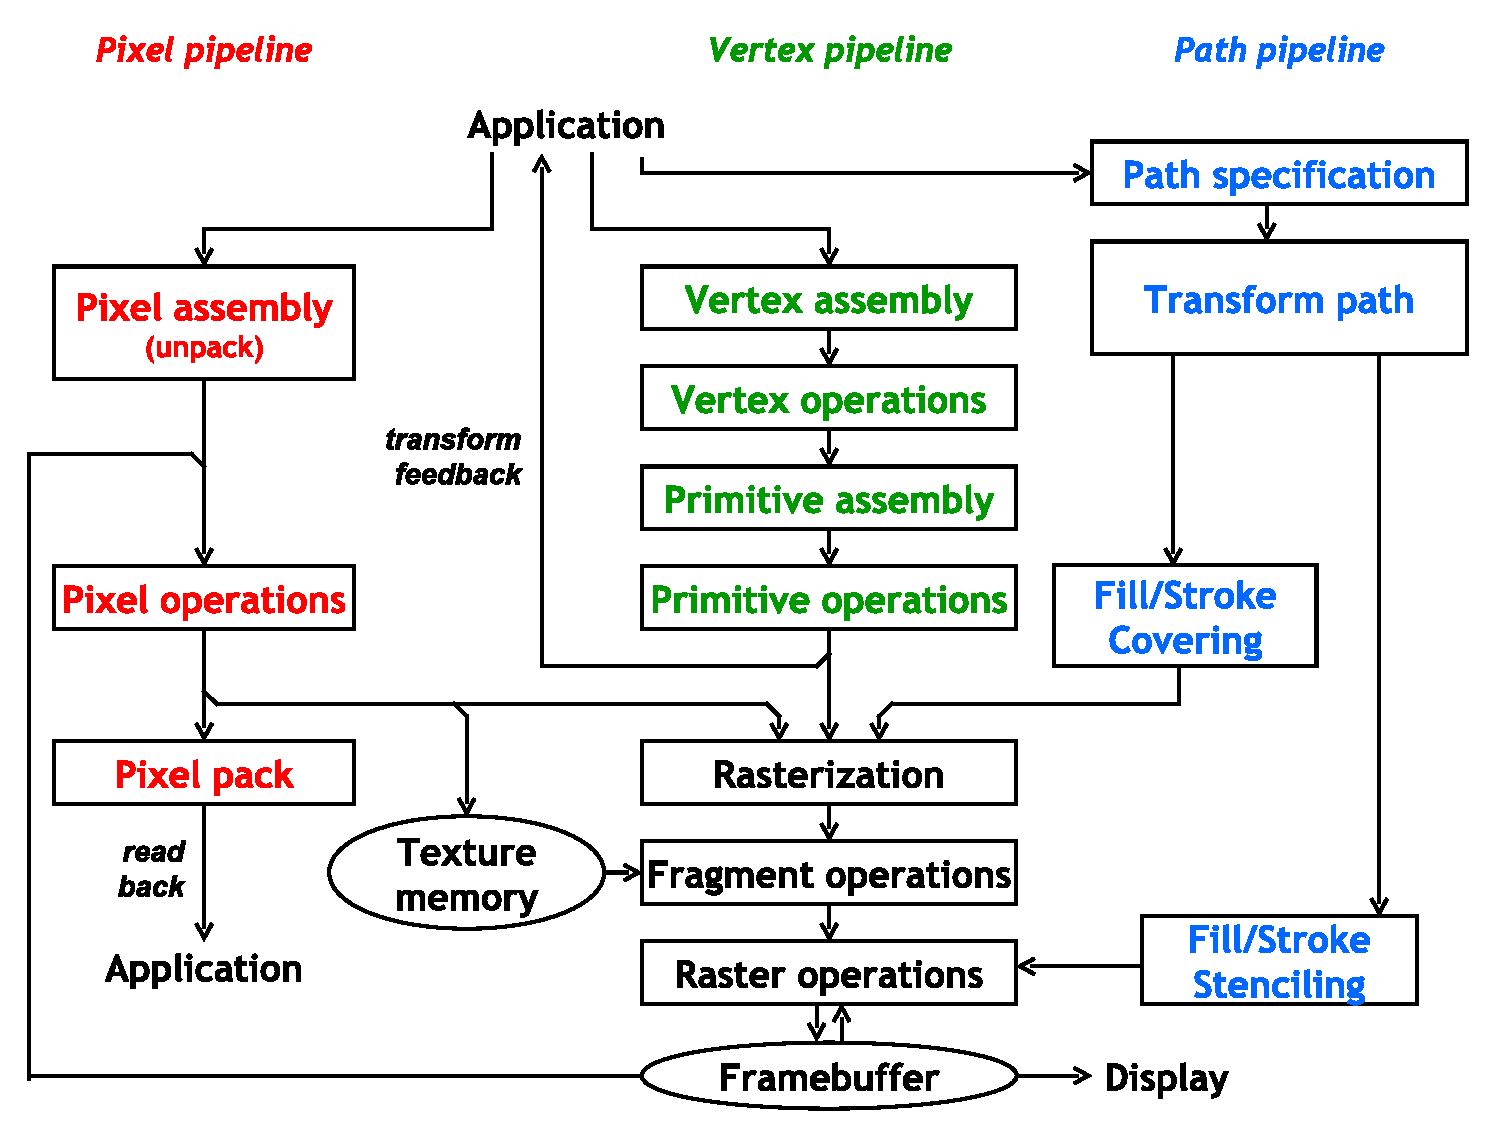
\includegraphics[width=\columnwidth]{pipelines.eps}}
  \center{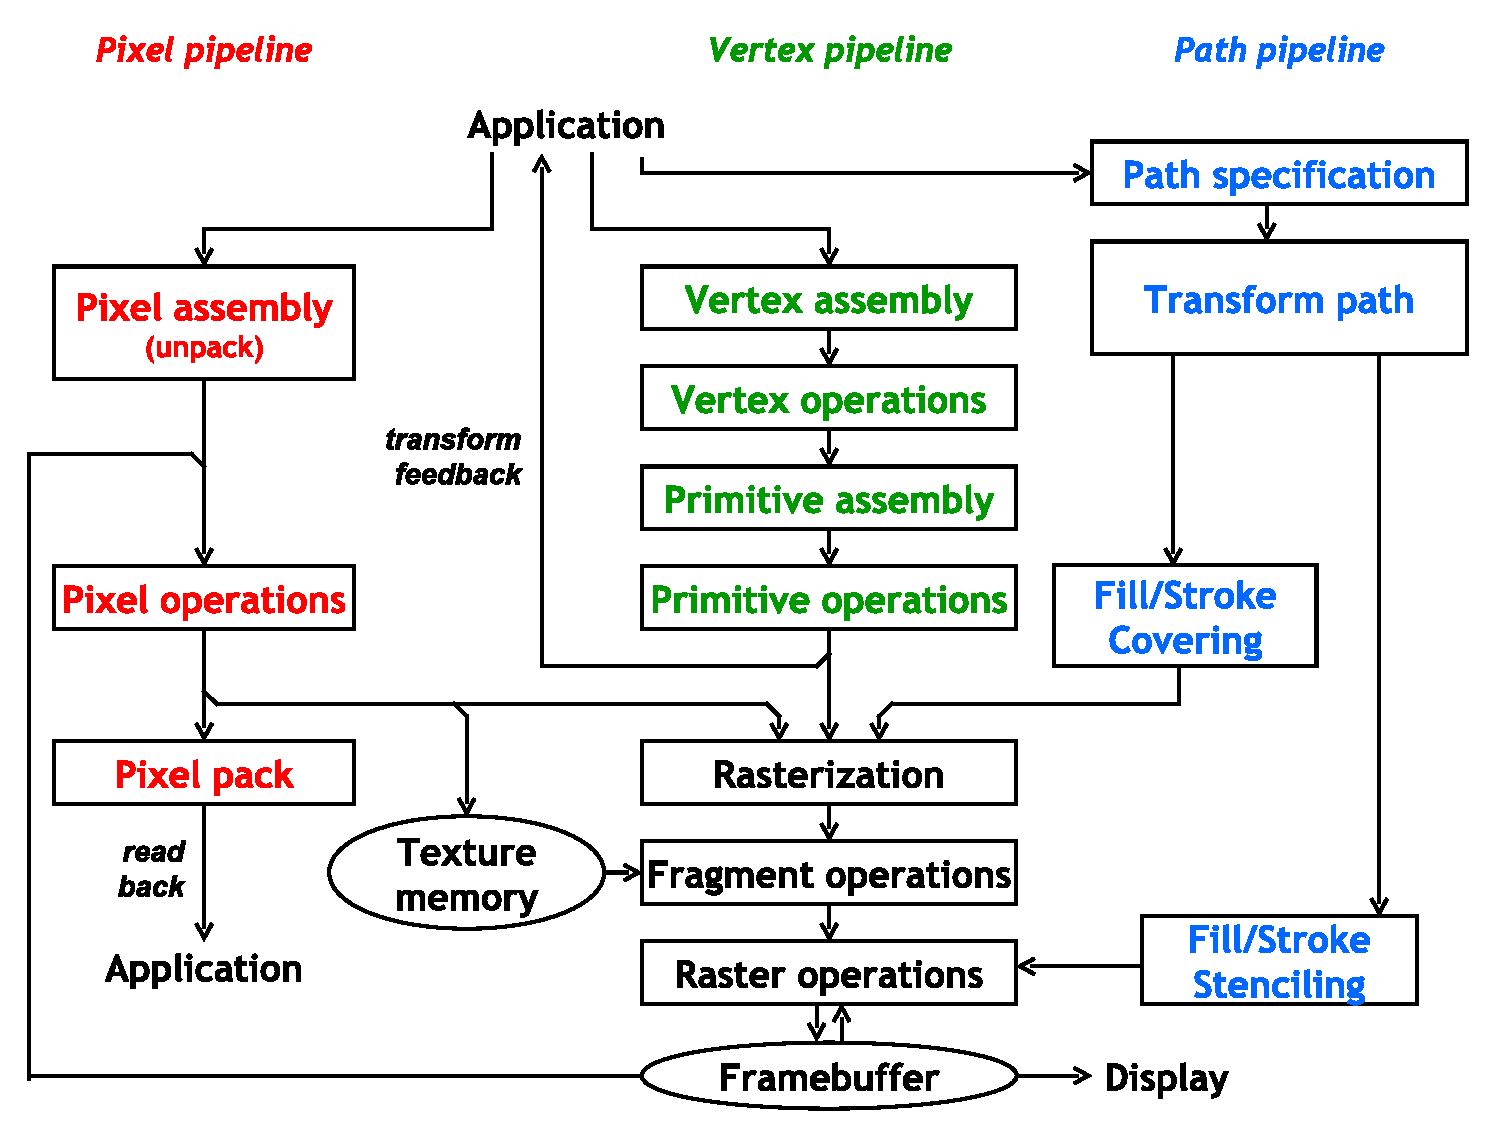
\includegraphics[width=\columnwidth]{pipelines.eps}}
  \caption{\label{fig:pipelines} High-level data flow of OpenGL showing
  pixel, vertex, and new path pipelines.}
\end{figure}

\subsection{Explicit Path Specification}

The command
\begin{lstlisting}
  void glPathCommandsNV(GLuint path,
                        GLsizei numCmds,
                        const GLubyte *cmds,
                        GLsizei numCoords,
                        GLenum coordType,
                        const void *coords);
\end{lstlisting}
specifies a new path object named {\em path} where {\em numCmds} indicates
the number of path commands, read from the array {\em commands}, with
which to initialize that path's command sequence.  These path commands
reference coordinates read sequentially from the {\em coords} array.
The type of the coordinates read from the {\em coords} array is determined
by the {\em coordType} parameter which must be one of {\tt GL\_BYTE}, {\tt
GL\_UNSIGNED\_BYTE}, {\tt GL\_SHORT}, {\tt GL\_UNSIGNED\_SHORT}, or {\tt GL\_FLOAT}.
Coordinates supplied in more compact data types allows paths to be stored
more efficiently.

The {\em numCmds} elements of the {\em cmds} array must be tokens (or
character aliases) from Table~\ref{tab:commands}.  The command sequence
matches the element order of the {\em cmds} array.  Each command
references a number of coordinates specified by the ``Number of scalar
coordinates'' column of Table~\ref{tab:commands}, starting with the first
(zero) element of the coords array and advancing by the coordinate count
for each command.

The following code fragment creates path object 42 containing the contours
of a five-point star and heart:
\begin{lstlisting}
  static const GLubyte pathCommands[10] =
    { GL_MOVE_TO_NV, GL_LINE_TO_NV,
      GL_LINE_TO_NV, GL_LINE_TO_NV,
      GL_LINE_TO_NV, GL_CLOSE_PATH_NV,
      'M', 'C', 'C', 'Z' };  // character aliases
  static const GLshort pathCoords[12][2] =
    { {100,180}, {40,10}, {190,120}, {10,120}, {160,10},
      {300,300}, {100,400}, {100,200}, {300,100},
      {500,200}, {500,400}, {300,300} };
  GLuint pathObj = 42;
  glPathCommandsNV(pathObj, 10, pathCommands,
    24, GL_SHORT, pathCoords);
\end{lstlisting}
The example demonstrates how tokens or character aliases can be used
interchangeably to specify a path.

\subsection{Grammars for Path Specification}

The command 
\begin{lstlisting}
  glPathStringNV(GLuint path, GLenum format,
                 GLsizei length, const void *pathString);
\end{lstlisting}
specifies a new path object named {\em path} where format must be either
{\tt GL\_PATH\_FORMAT\_SVG\_NV} or {\tt GL\_PATH\_FORMAT\_PS\_NV}, in which case the
{\em length} and {\em pathString} are interpreted respectively according to
SVG's grammar\footnote{The Backus-Naur Form (BNF) description of the SVG path grammar is found here \url{http://www.w3.org/TR/SVG/paths.html\#PathDataBNF}}
for paths or PostScript's sub-grammar for user paths.
This code fragment is functionally identical to the prior explicit path
specification example but uses an SVG path string:
\begin{lstlisting}
  const char *svgPathString =
    // star
    "M100,180 L40,10 L190,120 L10,120 L160,10 z"
    // heart
    "M300 300 "
    "C100 400,100 200,300 100,500 200,500 400,300 300Z";
  glPathStringNV(pathObj, GL_PATH_FORMAT_SVG_NV,
    (GLsizei)strlen(svgPathString), svgPathString);
\end{lstlisting}
Creating paths from strings has proven very convenient and avoids having
each application re-implement standard path grammar parsers.

\subsection{Specifying Paths from Glyphs of a Font}

Text rendering is a first-class feature in every major path rendering
API and standard.  Requiring applications to load outlines of glyphs
is just too common, not to mention arduous and platform-dependent,
so {\tt NV\_path\_rendering} provides a mechanism for applications to
create path objects from glyphs---including contiguous ranges of glyphs
indexed by their Unicode character points.

Two commands {\tt glPathGlyphRangeNV} and {\tt glPathGlyphsNV} create a sequence of path
objects given a font and a range or sequence of Unicode character points
for the font.  The font can be specified using a system font name (such as
``Arial'' or ``Helvetica'' with a file name for a file in a standard font
file format such as TrueType, or a built-in font name (such as ``Sans,''
``Serif,'' or ``Mono'') that is guaranteed to be available on every {\tt
NV\_path\_rendering} implementation, regardless of platform.

Once these path objects are populated, these glyph path objects can be
stenciled and covered, whether filled or stroked, just like any other
path object.

The {\tt glPathGlyphRangeNV} and {\tt glPathGlyphsNV} commands will only
create a path object for a given path name if that path object name
does \underline{not} already correspond to an existing path object.
This behavior is designed to populate path object ranges with glyph
outlines consistent with the {\tt font-family} property of CSS 2.1
\cite{CSS-Spec}.  An application can load a sequence of fonts for a
given range of path objects repeatedly knowing this will resolve to some
supported set of font glyphs eventually.

The {\tt glPathGlyphRangeNV} command has the following prototype:
\begin{lstlisting}
  void glPathGlyphRangeNV(GLuint firstPathName,
                          GLenum fontTarget,
                          GLconst void *fontName,
                          GLbitfield fontStyle,
                          GLuint firstGlyph,
                          GLsizei numGlyphs,
                          GLenum handleMissingGlyphs,
                          GLuint pathParameterTemplate,
                          GLfloat emScale);
\end{lstlisting}
The {\em emScale} parameter allows fonts of different formats to be loaded
with a consistent number of path units per em (a typographic measure of
glyph scale).\footnote{TrueType fonts user 2048 units for their em scale convention; PostScript fonts use 1000.  As most fonts today are based on TrueType conventions, using 2048 is a natural choice.}  Path coordinates and glyph metrics are scaled to match
the specified {\em emScale}.  To ensure all path objects in a range of glyphs
have a consistent set of path parameters, the {\em pathParameterTemplate} path
object names a path object from which the new glyph path objects should
copy their parameters.

This example shows how a range of path objects for sans serif fonts for
the Latin-1 character range can be populated:
\begin{lstlisting}
  // Constants
  const GLint numChars = 256;   // ISO/IEC 8859-1
                                // 8-bit range
  const GLfloat emScale = 2048; // TrueType path
                                // units per em
  
  // Create empty path object for use as parameter template
  GLuint pathTemplate = ~0;  // Biggest path name
  glPathCommandsNV(pathTemplate,
    0, NULL, 0, GL_FLOAT, NULL);
  glPathParameterfNV(pathTemplate,
    GL_PATH_STROKE_WIDTH_NV, emScale*0.1f);
  glPathParameteriNV(pathTemplate,
    GL_PATH_JOIN_STYLE_NV, GL_MITER_TRUNCATE_NV);
  glPathParameterfNV(pathTemplate,
    GL_PATH_MITER_LIMIT_NV, 1.0);
  // Create path object range for Latin-1 character codes
  GLuint glyphBase = glGenPathsNV(numChars);
  // Typeface names in priority order 
  struct {
    GLenum fontTarget;
    const char *name;
  } font[] = {
    { GL_SYSTEM_FONT_NAME_NV,   "Liberation Sans" },
    { GL_SYSTEM_FONT_NAME_NV,   "Verdana" },
    { GL_SYSTEM_FONT_NAME_NV,   "Arial" },
    // Final standard font provides guaranteed supported
    { GL_STANDARD_FONT_NAME_NV, "Sans" }
  };
  const int numFonts = sizeof(font)/sizeof(font[0]);
  for (int i=0; i< numFonts; i++) {  // For each font
    glPathGlyphRangeNV(glyphBase, 
      font[i].fontTarget, font[i].name, GL_BOLD_BIT_NV,
      0, numChars, GL_USE_MISSING_GLYPH_NV,
      pathTemplate, emScale);
  }
\end{lstlisting}
Path objects loaded from glyphs also have associated glyph and font
metrics loaded corresponding to their character point.  These metrics
and spacing information are discussed in Section~\ref{api:text}.

\subsection{Copied, Weighted, and Transformed Paths}

Additional commands for specifying path objects work by generating a new
path object from one or more existing path objects.  The {\tt glCopyPathNV}
command is the simplest and simply copies the state of a named existing
path object to another path object name.  Path parameters and glyph
metrics are copied by {\tt glCopyPathNV}.

The {\tt glInterpolatePathsNV} command takes two (source) path object names
and a weighting factor and creates a new (destination) path object
that is the linear interpolation based on the weighting factor of the
two source paths.  The {\tt glWeightPathsNV} command generalizes the {\tt
glInterpolatePathsNV} to linear combination of a specified number of source
path objects and corresponding weighting factors.  All the path objects
involved in interpolating or weighting must have identical path command
sequences and contain no circular or elliptical arc segment commands.
The destination path object's parameters are copied from the first
destination path object; glyph metrics are all set invalid (to -1).

The {\tt glTransformPathNV} command take a source path object name and
generates a new named destination path object corresponding to the
destination path object transformed by an affine linear transform.
Path commands such as horizontal or vertical lines or circular arcs may
be promoted to a more general path command form as required to perform
the transformation.  Relative commands are converted to absolute commands,
transformed, and then converted back to relative commands.

If the destination path object name refers to an existing path object,
that path object is replaced (implicitly deleting the old object) with the
new path object.  The destination name may be one of the source names.

Assuming the implementation performs a lazy copy of path commands and
coordinates, {\tt glCopyPathNV} allows efficient rendering of a path with
different stroking parameters.  {\tt glInterpolatePathsNV} can help implement
Flash's Shape Morph functionality and OpenVG's {\tt vgInterpolatePath}
command.  {\tt glTransformPathNV} can help implement SVG 1.2's non-scaling
stroke functionality and OpenVG's {\tt vgTransformPath}. 

\section{Path Parameters}
\label{api:parameters}

Every path object has state in addition to its sequence of path commands
and coordinates.

\subsection{Settable Parameters}

The {\tt glPathParameteriNV}, {\tt glPathParameterfNV}, {\tt glPathParameterivNV},
and {\tt glPathParameterfvNV} commands respectively set path parameters of
a specified path object given integer or float data supplied by a scalar
parameter or vector array.

Table~\ref{tab:parameters} summarizes the settable parameters.  Many
parameters deal with embellishments to stroking such as the stroke width,
join style, miter limit, end caps, and dash caps.
\begin{table}[htb]
\begin{center}
{\small
\begin{tabular}{|l|l|l|}
\hline
{\bf Name} & {\bf Type} & {\bf Initial value} \\
\hline
\hline
{\tt GL\_PATH\_STROKE\_WIDTH\_NV} & $\Re+$ & 1.0 \\
\hline
{\tt GL\_PATH\_JOIN\_STYLE\_NV} & 4-valued & {\tt GL\_MITER\_REVERT\_NV} \\
{\tt GL\_PATH\_MITER\_LIMIT\_NV} & $\Re+$ & 4 \\
\hline
{\tt GL\_PATH\_INITIAL\_END\_CAP\_NV} & 4-valued & {\tt GL\_FLAT} \\
{\tt GL\_PATH\_TERMINAL\_END\_CAP\_NV} & 4-valued & {\tt GL\_FLAT} \\
\hline
{\tt GL\_PATH\_INITIAL\_DASH\_CAP\_NV} & 4-valued & {\tt GL\_FLAT} \\
{\tt GL\_PATH\_TERMINAL\_DASH\_CAP\_NV} & 4-valued & {\tt GL\_FLAT} \\
{\tt GL\_PATH\_DASH\_OFFSET\_NV} & $\Re$ & 0.0 \\
{\tt GL\_PATH\_DASH\_OFFSET\_RESET\_NV} & 2-valued & {\tt GL\_MOVE\_TO\_CONTINUES\_NV} \\
\hline
{\tt GL\_PATH\_CLIENT\_LENGTH\_NV} & $\Re+$ & 0.0 \\
\hline
{\tt GL\_PATH\_FILL\_MODE\_NV} & 4-valued & {\tt GL\_COUNT\_UP\_NV} \\
{\tt GL\_PATH\_FILL\_MASK\_NV} & mask & all 1's \\
{\tt GL\_PATH\_FILL\_COVER\_MODE\_NV} & 3-valued & {\tt GL\_CONVEX\_HULL\_NV} \\
\hline
{\tt GL\_PATH\_STROKE\_COVER\_MODE\_NV} & 3-valued & {\tt GL\_CONVEX\_HULL\_NV} \\
{\tt GL\_PATH\_STROKE\_MASK\_NV} & mask & all 1's \\
\hline
\end{tabular}
}
\end{center}
\caption{Settable path object parameters.}
\label{tab:parameters}
\end{table}

\subsection{Dashing State}

Dashing is an embellishment to stroking where a repeated pattern of
enabled stroking and gaps in stroking is applied during stroking.
The conventional {\tt glPathParameteriNV}, etc. commands are ill-suited to
setting a variable number of dash offsets.

Instead parameters to control the dash pattern of a stroked path are
specified by the command
\begin{lstlisting}
  void glPathDashArrayNV(GLuint path,
                         GLsizei dashCount,
                         const GLfloat *dashArray);
\end{lstlisting}
where {\em path} is the name of an existing path object.  A {\em
dashCount} of zero indicates the path object is not dashed; in this case,
the {\em dashArray} is not accessed.  Otherwise, {\em dashCount} provides
a count of how many float values to read from the {\em dashArray} array.
The values provide an on/off pattern for dashing.  If the dash pattern is [3,1,3,2],
this indicates the dashing will repeat being on for 3 path-space units, off for 1
unit, on for 3 units, off for 2 units, etc.\footnote{An odd number of values ``doubles''
the specified pattern to make an even on/off pattern.}

\subsection{Computed Parameters and Querying State}

All settable path object state is able to be queried; this
includes settable parameters with {\tt glGetPathParameterivNV} and {\tt
glGetPathParameterfvNV}, the dashing array with {\tt glGetPathDashArrayNV},
the path command array with {\tt glGetPathCommandsNV}, and path coordinate
array with {\tt glGetPathCoordsNV}.  Additionally, computed parameters for
each path object can be queried; see Table~\ref{tab:computed}.
\begin{table}[htb]
\begin{center}
{\small
\begin{tabular}{|l|l|}
\hline
{\bf Name} & {\bf Type} \\
\hline
\hline
{\tt GL\_PATH\_COMMAND\_COUNT\_NV} & N \\
{\tt GL\_PATH\_COORD\_COUNT\_NV} & N \\
\hline
{\tt GL\_PATH\_COMPUTED\_LENGTH\_NV} & $\Re+$ \\
\hline
{\tt GL\_PATH\_OBJECT\_BOUNDING\_BOX\_NV} & $4\times\Re$ \\
{\tt GL\_PATH\_FILL\_BOUNDING\_BOX\_NV} & $4\times\Re$ \\
{\tt GL\_PATH\_STROKE\_BOUNDING\_BOX\_NV} & $4\times\Re$ \\
\hline
\end{tabular}
}
\end{center}
\caption{Computed path object parameters.}
\label{tab:computed}
\end{table}

\subsection{Glyph and Font Metrics}

Path objects created from character points from a font are tagged with
additional read-only glyph metrics.  These metrics are useful for text
layout.  Additionally, every glyph has aggregate per-font metrics for
its corresponding font.  The metrics are obtained directly from the font
except for any scaling based on the {\em emScale}.  The {\tt glGetPathMetricRangeNV}
and {\tt glGetPathMetricsNV} queries return the glyph and per-font metrics for a
range or sequence of path objects respectively.

As shown in Figure~\ref{fig:glyph-metrics}, the glyph metrics provide each
glyph's width and height and $(x,y)$ bearing and advance for both horizontal
and vertical layout.  These metrics are expressed in path space units.
 
\begin{figure}[b]
  \center{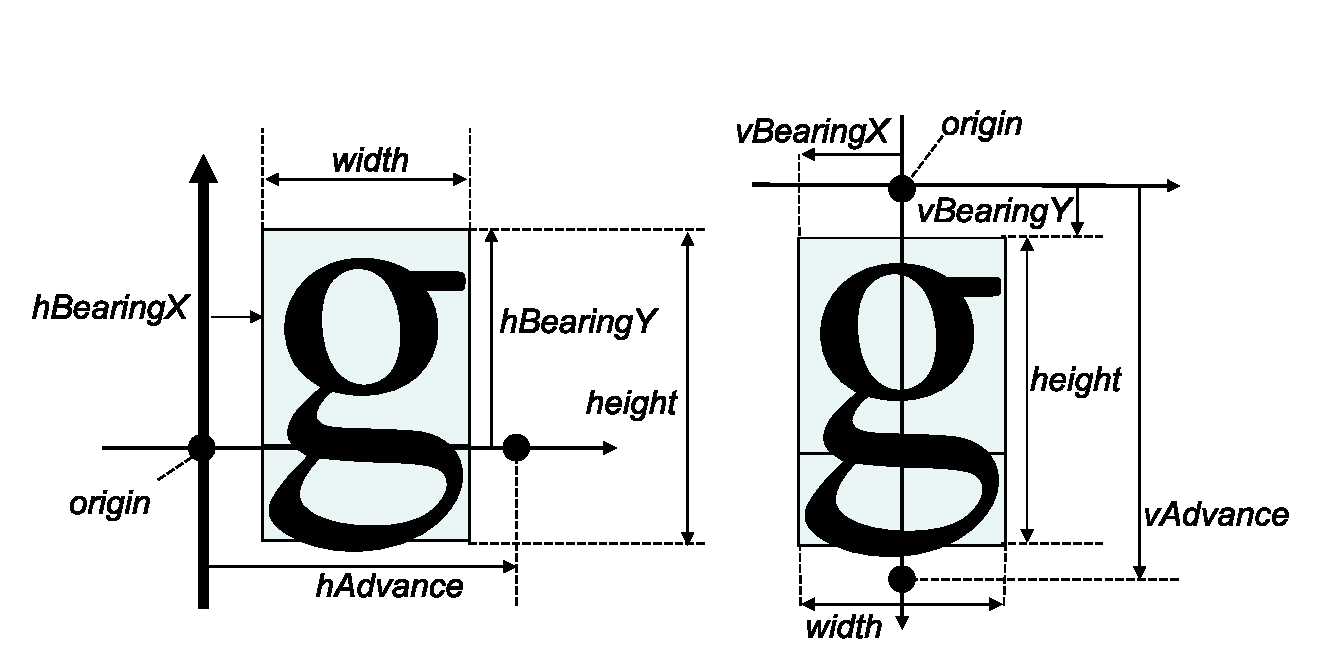
\includegraphics[width=\columnwidth]{glyph_metrics.eps}}
  \caption{\label{fig:glyph-metrics} Glyph metrics.}
\end{figure}

Additional per-font metrics can be queried from any glyph belonging to a
particular font.  These metrics include a bounding box large enough to
contain any glyph in the font, the native number of font units per em,
the font-wide ascender, descender, and height distances, maximum advance
for horizontal and vertical layout, underline position and thickness.

Requested metrics are specified in a bitmask and returned to an
application-provided array of floats.

\section{Rendering Paths via Stencil, then Cover}

Once a path object is created, it can be rendered with the ``stencil,
then cover'' approach.

The mapping from path space to clip space and ultimately window space
is determined by OpenGL's standard modelview, projection, viewport,
and depth range transforms.  An OpenGL programmer familiar with OpenGL's
{\tt glMatrixMode}, {\tt glRotatef}, {\tt glTranslatef}, etc. matrix commands
for transforming 3D geometry uses the same commands to manipulate the
transformations of path objects.

For example, the code below establishes an orthographic path-to-clip-space
to map the $[0..500]\times[0..400]$ region used by the star-and-heart path:
\begin{lstlisting}
  glMatrixLoadIdentityEXT(GL_PROJECTION);
  glMatrixLoadIdentityEXT(GL_MODELVIEW);
  glMatrixOrthoEXT(GL_MODELVIEW, 0, 500, 0, 400, -1, 1);
\end{lstlisting}
This code demonstrates OpenGL's selector-free matrix manipulation
commands introduced by the {\tt EXT\_direct\_state\_access} (DSA) extension \cite{DSA}.

\subsection{Path Rendering in Two Steps}

Now we can render the filled and stroked star-and-heart path.  We assume
the stencil buffer has been initially cleared to zero.

\paragraph{Stencil Step for Filling}

First we stencil the filled region of the star-and-heart path into the
stencil buffer with the {\tt glStencilFillPathNV} command:
\begin{lstlisting}
  glStencilFillPathNV(pathObj, GL_COUNT_UP_NV, 0x1F);
\end{lstlisting}
The winding number of each sample in the framebuffer w.r.t. the
transformed path is added ({\tt GL\_COUNT\_UP}) to the stencil value corresponding
to each rasterized same.   The 0x1F mask indicates that only the five
least significant stencil bits are modified---effectively resulting in
modulo-32 addition.  More typically, this mask will be 0xFF.

Instead of {\tt GL\_COUNT\_UP}, we could also subtract ({\tt GL\_COUNT\_DOWN})
or invert bits ({\tt GL\_INVERT}) by a count equal to each sample's winding
number w.r.t. the transformed path.

\paragraph{Cover Step for Filling}

Second we conservatively cover the previously stenciled filled region
of the star-and heart path.  The shading, stencil testing, and blending
are fully controlled by the application's OpenGL context state during
the cover.  So we first enable stencil testing to discard color samples
with a stencil value of zero (those not in the path as determined by
the prior stencil step); for samples that survive the stencil test,
we want to reset the stencil value to zero and shade the corresponding
sample's color value green.  So:
\begin{lstlisting}
  glEnable(GL_STENCIL_TEST);
  glStencilFunc(GL_NOTEQUAL, 0, 0x1F);
  glStencilOp(GL_KEEP, GL_KEEP, GL_ZERO);
  glColor3f(0,1,0); // green
  glCoverFillPathNV(pathObj, GL_BOUNDING_BOX_NV);
\end{lstlisting}
The result is a green star to the left of a green heart.  A single cover step
updates any particular color sample no more than once; this ensures against
double blending of color samples--as required by path rendering standards.

\paragraph{Stencil Step for Stroking}

Stroking proceeds similarly in two steps; however before rendering, we
configure the path object with desirable path parameters for stroking.
Specify a wider 6.5-unit stroke and the round join style:
\begin{lstlisting}
  glPathParameteriNV(pathObj,
    GL_PATH_JOIN_STYLE_NV, GL_ROUND_NV);
  glPathParameterfNV(pathObj,
    GL_PATH_STROKE_WIDTH_NV, 6.5);
\end{lstlisting}
Now we first stencil the stroked coverage for the heart-and-star path
into the stencil buffer:
\begin{lstlisting}
  glStencilStrokePathNV(pathObj, 0x1, ~0);
\end{lstlisting}
This computes the point containment of every sample in the framebuffer
w.r.t. the stroked path---and if the sample is contained in the path's
stroke, the sample's stencil value is set to 0x1 with a write mask of bit-inverted zero
(writing all stencil bits).

\begin{figure}[tb]
  \center{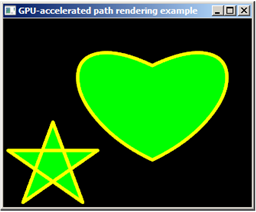
\includegraphics[width=\columnwidth]{star_and_heart.png}}
  \caption{\label{fig:star-and-heart} Filled and stroked path rendering result.}
\end{figure}

\paragraph{Cover Step for Stroking}

Second we conservatively cover the previously stenciled stroked
region of the star-and heart path.  We leave stencil as configured
previously---non-zero values will include the 0x1 value written by the
{\tt glStencilStrokePathNV} command, but we change the color to yellow:
\begin{lstlisting}
  glColor3f(1,1,0); // yellow
  glCoverStrokePathNV(pathObj, CONVEX_HULL);
\end{lstlisting}
The complete rendering result is shown in Figure~\ref{fig:star-and-heart}.

\subsection{Accessible Samples}

The fill and stroke stencil/cover commands {\em conceptually} operate
on all samples in the framebuffer.  Potentially every sample in the
framebuffer could be updated by these commands.  However, the set of {\em
accessible samples} may be restricted the by current OpenGL context state.

Clip planes, polygon stipple, window ownership, scissoring, stencil
testing (on write masked stencil bits during stencil fill/stroke
operations), depth testing, depth bounds testing, and the multisample
mask all limit, when enabled, the accessible samples.

The cover fill/stroke commands further limit the updated samples to the
bounding box or convex hull (depending on the cover mode). 

\subsection{Path Coordinate Generation}

Paths do not have per-vertex attributes such as colors and texture
coordinates that are interpolated over geometric primitives as 3D
geometry does.  Instead varying attributes used by the fragment shader
must be generated as a linear function of the path-space coordinate
system.  The {\tt glPathColorGenNV}, {\tt glPathTexGenNV}, and {\tt glPathFogGenNV}
command generated color, texture coordinate sets, and the fog coordinate
respectively; these loosely mimic OpenGL's fixed-function {\tt glTexGenfvNV},
etc. commands.

For example, to match a common idiom in path rendering standards, the path coordinate
generation supports mapping a path's path space bounding box to a
normalized $[0..1]\times[0..1]$ square.  To apply a 4x3 tile pattern stored in
a repeated 2D texture to the bounding box extents of a covered path, 
configure path texture coordinate generation this way:
\begin{lstlisting}
  const GLfloat coeffs[4] = { 1.0/4, 0,   // s = x/4 + 0
                              1.0/3, 0 }  // t = y/3 + 0
  GLint numCoordinates = 2;  // for s and t
  GLenum texUnit = GL_TEXTURE0;
  glPathTexGenNV(texUnit, GL_PATH_OBJECT_BOUNDING_BOX_NV,
    numCoordinates, coeffs);
  glActiveTexture(texUnit);
  glEnable(GL_TEXTURE_2D);
\end{lstlisting}

\section{Text Handling}
\label{api:text}

\subsection{Instanced Rendering}

Efficient rendering of glyphs is very important for any path rendering
system.  In addition to the ability to create path objects from Unicode
character points of fonts and query glyph metrics for such path objects,
instanced commands for stenciling and covering sequences of path objects
in a single OpenGL command are provided.

{\tt glStencilFillPathInstancedNV} and {\tt glCoverFillPathInstancedNV}
for filling and {\tt glStencilStrokePathInstancedNV} and {\tt
glCoverStrokePathInstancedNV} for stroking accept arrays of path objects
where each path object instance has its own local transformation.

This is intended for rendering spans of characters with corresponding
glyph path objects, but could be used for rendering any sequence of
path objects.  To facilitate text, there is a base path object value to
which each path object offset in the sequence is added.  This allows a
string of ASCII characters to be provided where the base path object
value identifies the base of a range of glyphs specified with {\tt
glPathGlyphRangeNV}.  The array of offsets can even be a UTF-8 or UTF-16
string to facilitate easy rendering of Unicode text.

The instanced cover commands include a special
{\tt GL\_BOUNDING\_BOX\_-OF\_BOUNDING\_BOXES} cover mode where the bounding boxes
of each locally transformed path object's cover geometry is combined
({\em unioned}) into a single bounding box.

These instanced commands give the OpenGL implementation the freedom to
reorder the geometry sets used during the instanced stencil step for
better efficiency in the GPU.  

\subsection{Spacing and Kerning}

Good aesthetics and legibility for horizontal spans of text generally
involves appropriate spacing for the glyphs.  When this spacing depends
on which pairs of glyphs are mutually adjacent, this is called kerning.
We provide a {\tt glGetPathSpacingNV} query that accepts a sequence of path objects
(in the same way the instanced stencil/cover commands do) and returns an
array of translations corresponding to the kerned spacing of the glyphs.

The returned array of translations from {\tt glGetPathSpacingNV} is immediately
suitable to pass as the array of translations used for the local
transformation sequence when using the instanced stencil/cover commands.

While applications with complex text layout requirements might judge this
mechanism insufficiently sophisticated, because the mechanism is simple,
cross-platform, and generates kerned glyph translations as expected by
the instanced stencil/cover commands, we anticipate this functionality
will meet the basic text layout needs of many applications.

\section{Geometric Queries}

{\tt NV\_path\_rendering} includes a set of common geometric queries on
paths.  The queries {\tt glIsPointInFillPathNV} and {\tt glIsPointInStrokePathNV} provide
efficient determinations of whether an $(x,y)$ point in a path's local
coordinate system is inside or outside the fill or stroke of the path.
The query {\tt glGetPathLengthNV} provides a means to obtain arc lengths over
specified command sequences for a path.  The query {\tt glPointAlongPathNV}
returns an $(x,y)$ point and $(dx,dy)$ tangent a given arc length into a
path's command sequence.

These queries are intended to be compatible with queries supported by OpenVG.

The crucial rationale for these queries is they are consistent with
our implementation's internal computations for being inside/outside the
path's stroke or fill and arc length computations (such as for dashing).

\section{Antialiasing}

Applications are expected to render into multisample framebuffers to achieve
acceptable antialiasing quality.  Use existing APIs to allocate multisample
framebuffer resources.  {\tt NV\_path\_rendering} automatically generates multisample
coverage when the framebuffer supports multisampling.

Applications can also use OpenGL's accumulation buffer mechanism with jittered
rendering to exceed the base multisampling quality available.
